\documentclass[11pt,letterpaper]{article}

\usepackage[margin=1in]{geometry}
\usepackage[T1]{fontenc}
\usepackage{mathptmx}
\usepackage{microtype}
\usepackage{amsmath,amssymb}
\usepackage{booktabs,threeparttable,array,tabularx}
\usepackage{graphicx,float,placeins}
\usepackage[font=small,labelfont=bf,labelsep=colon,skip=6pt]{caption}
\usepackage{natbib}
\usepackage{hyperref}
\usepackage{xcolor}
\usepackage{setspace}

\setstretch{1.12}
\setlength{\parindent}{1.5em}
\setlength{\parskip}{0pt}
\setlength{\textfloatsep}{14pt plus 3pt minus 2pt}
\setlength{\floatsep}{12pt plus 3pt minus 2pt}
\renewcommand{\arraystretch}{1.12}
\setlength{\tabcolsep}{5pt}
\graphicspath{{../output/figures/}}
\hypersetup{
  colorlinks=true,
  linkcolor=black,
  citecolor=blue!45!black,
  urlcolor=blue!45!black,
  pdftitle={Who Bears the Error?},
  pdfauthor={Zhixun Zheng}
}

\title{\textbf{Who Bears the Error?}\\[5pt]
\large Threshold Choice, Fairness Trade-offs, and Institutional Accountability in COMPAS}
\author{Zhixun Zheng}
\date{August 2026}

\begin{document}
\maketitle

\begin{abstract}
Using ProPublica's historical Broward County COMPAS data, this study asks how a common classification threshold redistributes observed false-positive and false-negative errors across recorded racial groups. It reproduces published two-year contingency counts in the full 7,214-defendant sample, evaluates all common decile thresholds, estimates pointwise uncertainty with 5,000 race-stratified defendant-level bootstrap replicates, and applies prespecified asymmetric error-loss analyses in the 6,150-defendant Black-White comparison sample. Black and White ROC AUC values were nearly identical (0.6918 and 0.6931), but at $t=5$ their false-positive rates were 44.85\% and 23.45\%, and their false-negative rates were 27.99\% and 47.72\%. Under per-defendant loss, false-positive weights of $\lambda=.25,.50,.75$ selected thresholds $t^*=2,6,10$; at equal weighting, a prespecified class-conditional loss instead selected $t=5$. Moving from $t=5$ to $t=6$ in the comparison sample exchanged 319 fewer false positives for 287 more false negatives. These are comparisons of analytical rules, not estimates of their effects in actual judicial decisions. The results make three choices available for institutional scrutiny: the threshold, the definition and weighting of error, and the consequence attached to a classification.
\end{abstract}

\noindent\textbf{Keywords:} COMPAS; algorithmic fairness; classification thresholds; false positives; false negatives; institutional accountability

\section{Introduction}

ProPublica's COMPAS investigation reported that, among Broward County defendants who were not rearrested within two years, Black defendants were nearly twice as likely as White defendants to be classified above the low-risk category; false-negative rates ran in the opposite direction \citep{angwin2016,larson2016}. A subsequent reanalysis found similar Black and White ranking discrimination and approximately similar observed rearrest rates within broad score categories \citep{flores2016}. These findings describe different properties of the scores. AUC concerns ranking, PPV the composition of a classified group, and FPR and FNR the two directions of classification error. Under unequal observed outcome rates and imperfect prediction, plausible fairness criteria can conflict \citep{chouldechova2017,kleinberg2017}.

The dispute also raises a decision question that no performance metric answers alone. A graded score does not specify where to draw a binary cutoff or what a higher-risk classification should be allowed to influence. The selected threshold changes who falls into each category, while the chosen loss function determines which errors count most in an optimization. This paper asks: How does a common threshold redistribute observed false-positive and false-negative errors across recorded racial groups in historical COMPAS data, and which choices must an institution account for when using such a rule?

The analysis reproduces ProPublica's published two-year contingency counts, sweeps every common decile threshold, estimates Black-minus-White metric gaps with 5,000 race-stratified defendant-level bootstrap replicates, and evaluates prespecified error-loss specifications. Black and White AUC values are nearly identical, yet FPR and FNR gaps remain oppositely signed across interior thresholds. Under the primary per-defendant loss, changing the false-positive weight from $\lambda=.25$ to $.50$ to $.75$ moves the aggregate optimum from $t=2$ to $t=6$ to $t=10$. At $\lambda=.50$, changing the loss normalization alone moves the optimum from $t=6$ to $t=5$.

The known-result replication and bootstrap provide checks for two focused comparisons: the exchange of errors between adjacent thresholds, and the different optima produced by two prespecified loss definitions at the same numerical weight. These comparisons motivate a limited institutional proposal: record the rule, the alternatives, the consequence it may influence, and the reasons for choosing it. The historical scores and observed two-year rearrest labels do not reveal which thresholds officials used or what effects a classification had on an individual's legal outcome. Section 2 reviews the relevant empirical and legal debate; Sections 3 and 4 present the design and results; Section 5 develops the proposed accountability record.

\section{Background and Related Work}

\subsection{The COMPAS dispute and competing empirical interpretations}

The public COMPAS debate began from a disagreement about what property of a risk instrument should count as evidence of fair performance. ProPublica examined Broward County defendants with two years of follow-up and reported sharply different directions of error at the Low versus Medium/High cutoff: Black defendants who were not rearrested were classified above Low more often than White defendants, while White defendants who were rearrested were classified Low more often than Black defendants \citep{angwin2016,larson2016}. Northpointe's response disputed ProPublica's interpretation and organized its defense around accuracy equity and predictive parity, while also objecting to aspects of the cutoff and error analysis \citep{dieterich2016}.

\citet{flores2016} offered a related but distinct reanalysis. Using the decile score and a more restricted analytical sample, they reported AUC values of 0.69 for White defendants and 0.70 for Black defendants, with no statistically significant difference, and observed rearrest rates that were close across the two groups within the broad Low, Medium, and High categories. They also emphasized that converting a three-category instrument into a binary classifier requires a binning decision. The two binning rules they examined changed false-positive and false-negative rates in opposite directions.

These analyses answer different statistical questions and, in places, use different samples. Similar ranking discrimination or outcome rates within broad score categories do not imply equal false-positive and false-negative rates after a cutoff is imposed. Conversely, unequal classification-error rates do not by themselves establish different ranking discrimination across groups. The present analysis therefore reports AUC, PPV, FPR, and FNR as distinct properties rather than treating any one metric as a complete fairness verdict. It reproduces the published contingency table as a known result and treats the threshold as an explicit analytical input.

\subsection{Different metrics answer different questions}

The relevant measures condition on different events. ROC AUC describes how often a randomly selected rearrested defendant receives a higher score than a randomly selected non-rearrested defendant, counting a score tie as one-half. It is a ranking measure and does not require a particular threshold. Positive predictive value instead conditions on the higher-risk classification and asks what share of those classified higher risk were observed to be rearrested. False-positive and false-negative rates condition on the observed outcome and distinguish the two directions of error.

Because the denominators differ, parity on one measure does not imply parity on another. This point is especially important when a score is used in a decision process. AUC concerns the ordering produced by the score; PPV concerns the composition of a selected category; FPR and FNR concern who bears each type of classification mistake. Reporting them together is therefore not a search for one master fairness statistic. It is an accounting of distinct properties that may matter for distinct institutional reasons.

\subsection{Calibration, predictive parity, and incompatibility}

\citet{chouldechova2017} formalized the relationship among prevalence, predictive parity, and classification-error rates. When observed outcome prevalence differs across groups, equal PPV at a threshold is generally incompatible with equal FPR and FNR unless prediction is perfect. Her COMPAS illustration also showed that approximate calibration or predictive parity can coexist with error-rate imbalance. The result explains why ProPublica and its critics could emphasize different, statistically defensible properties of the same data.

\citet{kleinberg2017} established a related score-level result. They considered calibration within groups, balance for the negative class, and balance for the positive class, and showed that all three can be satisfied together only in constrained cases: perfect prediction or equal base rates. Their balance conditions are score-level conditions, not identical to threshold-specific FPR and FNR parity, although they generalize the same concern about differential treatment of positive and negative classes.

Neither theorem chooses an institutional objective. Kleinberg and colleagues expressly declined to recommend how conflicts among fairness definitions should be resolved, and Chouldechova distinguished statistical criteria from the social and ethical judgment of fairness. Here, the incompatibility results provide context for the empirical pattern and clarify why metric trade-offs remain after a common threshold is chosen.

\subsection{From a score to a decision rule}

The distinction between a score and a rule is already visible in the early COMPAS exchange. \citet{flores2016} observed that a multicategory score must be binned before contingency-table measures can be calculated. They showed that placing Medium with High lowers one type of error and raises another relative to placing Medium with Low, and noted that different users could prefer different trade-offs. ProPublica likewise reported its main Low-versus-Medium/High table and a High-only sensitivity check \citep{larson2016}.

Those comparisons identify the threshold as consequential, but they do not map the full available threshold space or make the weighting of false positives and false negatives explicit. This study adds that step. It evaluates every common decile threshold, reports uncertainty across the resulting metric curves, and asks how a transparent loss-minimizing threshold changes when the relative error weight changes. This study therefore audits the choices required to turn an existing score into a common binary rule.

\subsection{Institutional use and contestability}

The legal controversy surrounding COMPAS also illustrates why predictive evaluation does not settle legitimate use. In \textit{State v. Loomis}, the Wisconsin Supreme Court held that a sentencing court's consideration of COMPAS did not violate due process when the assessment was used with the limitations and cautions specified in the opinion \citep[paras. 98--100, 120]{loomis2016}. The holding was narrow. The court said that a risk score could not determine incarceration or sentence severity, could not be the determinative factor in deciding whether community supervision was safe and effective, and had to be accompanied by a written advisement addressing the proprietary model, group-based inference, possible racial disparity, the absence of Wisconsin cross-validation at the time, and the need for continuing monitoring. The court also stressed that the sentencing judge had relied on independent factors and stated that the sentence would have been the same without COMPAS \citep[paras. 104--109]{loomis2016}.

\textit{Loomis} therefore should not be cited as a general judicial endorsement of COMPAS or as proof that a particular threshold is lawful. It shows, within one jurisdiction and procedural setting, that the authority given to a score depends on the permitted consequence, the reasons independently supporting the decision, the warnings supplied to the decision-maker, and the opportunity to review and challenge relevant information. The accountability framework developed here is a normative proposal informed by those concerns, not a claim that its four modules exhaust constitutional or statutory requirements.

Together, this literature leaves a focused gap. Prior work explains competing metrics, demonstrates incompatibilities, and identifies legal cautions around institutional use. It does not, by itself, show how every available common threshold redistributes observed errors, how sampling uncertainty surrounds that redistribution, or how prespecified error weights move the aggregate optimum. Those are the empirical steps used below to connect score evaluation to institutional responsibility.

\section{Data and Methods}

\subsection{Data source and provenance}

The analysis used ProPublica's public \texttt{compas-scores-two-years.csv} file from the \texttt{propublica/compas-analysis} repository \citep{larson2016}. The source was fixed at commit \texttt{bafff5da3f2e45eca6c2d5055faad269defd135a}; the downloaded file had SHA-256 digest \texttt{c451db85908b2f7fef1d83203bedf6b71ecda0d5af468d82ae62178f91d0cc7d} and dimensions 7,214 rows by 53 columns. The data concern defendants scored in Broward County, Florida, principally during 2013--2014. The pipeline downloaded the commit-pinned file and halted before analysis if its checksum or dimensions differed from these frozen values.

Additional integrity checks required the outcome to be binary, the general recidivism score to lie from 1 through 10, the defendant identifier to be unique and complete, and the analysis variables to contain no missing values. The raw CSV contains two columns headed \texttt{decile\_score}; after import, the second is named \texttt{decile\_score.1}. The preparation step required these columns to agree in all rows before retaining one as the canonical general recidivism score. The violent-risk variable \texttt{v\_decile\_score} was not used. Any failed check halted the pipeline rather than triggering silent row deletion or imputation.

The source file contains direct identifiers and detailed case fields that were unnecessary for the analysis. Neither the raw file nor any row-level processed table was retained in the public repository. If generated at runtime, the minimized table contained only a nonidentifying row key, recorded race, general recidivism decile score and category, and the two-year outcome, and was excluded through \texttt{.gitignore}. Public machine-readable outputs were limited to aggregated figure-source and result tables. The pinned download, checksum, and preparation code therefore provide reproducibility without republishing a second person-level dataset.

\subsection{Analysis populations and variables}

The known-result replication used sample R, all 7,214 rows in the source file: 3,696 recorded as \texttt{African-American}, 2,454 as \texttt{Caucasian}, 637 as Hispanic, 377 as Other, 32 as Asian, and 18 as Native American. It did not apply the separate 30-day case-matching filters used in some other parts of ProPublica's analysis because the published two-year error tables were calculated from the full file. The primary comparative sample C contained the 6,150 defendants recorded as \texttt{African-American} or \texttt{Caucasian}. These categories are displayed as Black and White for readability, but they are administrative labels in the source data rather than measures of self-identified racial identity. The smaller recorded groups were included in the replication audit and pooled estimates but excluded from the prespecified two-group comparisons.

For defendant $i$, $Y_i=1$ denoted \texttt{two\_year\_recid = 1}, and $Y_i=0$ otherwise. This variable measures observed rearrest within two years, not true offending. The general recidivism decile score was denoted $S_i\in\{1,\ldots,10\}$, and the focal recorded group was $G_i\in\{B,W\}$. No values of the score, outcome, or race variables were imputed.

\subsection{Threshold rules and performance measures}

For each common threshold $t$, the analytical binary rule was
\[
\widehat{Y}_{i,t}=\mathbf{1}(S_i\ge t),
\qquad t\in\{1,2,\ldots,11\}.
\]
Thus, $t=1$ classified every defendant as higher risk, whereas $t=11$ classified none. The $t=5$ rule reproduced COMPAS Low versus Medium/High, and $t=8$ reproduced Low/Medium versus High. Every primary comparison applied the same threshold to all groups. The endpoint rules were retained to display the full available decision space; a metric with an empty denominator was stored as undefined rather than set to zero.

At each threshold, true-negative, false-positive, false-negative, and true-positive counts were computed before the corresponding rates. The primary metrics were
\[
FPR=\frac{FP}{FP+TN},\qquad
FNR=\frac{FN}{FN+TP},\qquad
PPV=\frac{TP}{TP+FP}.
\]
The primary group contrasts were signed Black-minus-White differences in these rates. Differences rather than ratios were used as the primary contrasts because ratios become unstable when the White reference rate approaches zero; Black/White FPR and FNR ratios were retained only for the two prespecified reference cutoffs, $t=5$ and $t=8$. The threshold sweep also calculated TPR, TNR, NPV, selection rate, accuracy, balanced accuracy, and overall error rate, with the underlying numerators and denominators retained in the canonical outputs.

Threshold-independent ranking discrimination was summarized by the empirical ROC AUC for sample R, Black defendants, White defendants, and the signed Black-minus-White difference. AUC was interpreted as a ranking measure, not as evidence that classification errors at a selected cutoff were similar. As a descriptive score-level calibration diagnostic, the analysis also estimated
\[
q_{g,s}=P(Y=1\mid S=s,G=g),
\]
for each score $s=1,\ldots,10$, together with $q_{B,s}-q_{W,s}$. Because the COMPAS decile is not a literal predicted probability, no Brier score or probability-calibration slope was calculated from $S/10$.

\subsection{Bootstrap uncertainty}

Uncertainty was evaluated with 5,000 nonparametric defendant-level bootstrap replicates generated by NumPy's \texttt{PCG64} generator with seed \texttt{20260807}. For sample C comparisons, defendants were resampled with replacement within the Black and White groups separately, preserving both observed group sizes. For pooled sample-R estimates, resampling occurred within all six recorded race categories, preserving the observed race composition. Each replicate recomputed the threshold-dependent metrics and signed gaps, pooled and group-specific AUC values, score-level rearrest rates, and the focal error-cost optima.

Intervals were the 2.5th and 97.5th percentiles of the bootstrap distribution. Threshold and score curves use pointwise, not simultaneous, 95\% intervals and were not interpreted as a sequence of significance tests. A replicate-specific undefined value was stored as missing, and an interval was suppressed if fewer than 95\% of replicates produced a defined estimate.

\subsection{Error-cost sensitivity}

The primary sensitivity analysis evaluated the per-defendant aggregate loss in sample C,
\[
L_t(\lambda)=\frac{\lambda FP_t+(1-\lambda)FN_t}{N},
\qquad \lambda\in[0,1],
\]
where $\lambda$ is the prespecified weight on a false positive and $1-\lambda$ is the weight on a false negative. Loss was calculated for all thresholds and for $\lambda=0,0.01,\ldots,1$. For each value of $\lambda$, the estimand was the complete minimizing set
\[
T^*(\lambda)=\underset{t\in\{1,\ldots,11\}}{\arg\min}\;L_t(\lambda).
\]
All tied minimizers were retained. When a display required one line, the highest minimizing threshold was shown as an explicit convention favoring fewer higher-risk classifications, not as an additional optimization criterion. The focal values $\lambda=0.25,0.50,0.75$ represent false-positive to false-negative weight ratios of 1:3, 1:1, and 3:1.

To examine the distribution associated with an aggregate optimum, group-specific weighted error loss was defined as
\[
L_{g,t}(\lambda)
=\lambda\frac{FP_{g,t}}{N_g}+(1-\lambda)\frac{FN_{g,t}}{N_g}.
\]
This quantity was evaluated at $t=5$, $t=8$, and the focal minimizing thresholds. It is a modeled sensitivity quantity rather than a measurement of realized social harm. In the bootstrap, the analysis recorded how often each threshold belonged to the full minimizing set at each focal $\lambda$. Because a replicate could contain tied minimizers, membership frequencies across thresholds need not sum to 100\%.

As a prespecified robustness check, the optimization was repeated using the class-conditional loss
\[
\widetilde{L}_t(\lambda)=\lambda FPR_t+(1-\lambda)FNR_t.
\]
Unlike the per-defendant primary loss, this expression gives equal structural weight to the non-rearrested and rearrested conditional pools before applying $\lambda$. Comparing the two specifications makes visible the dependence of an optimum on both the chosen error weights and population base rates. Neither loss function estimates which weighting is legally, morally, or institutionally appropriate.

\subsection{Prespecification and reproducibility}

The analysis plan was frozen before implementation of the threshold, bootstrap, and cost extensions. Because the dataset was public and ProPublica's headline error rates were already known, the $t=5$ analysis was designated a known-result replication rather than a blind preregistration. Extension results were generated only after the acquisition and integrity checks passed and the expected $t=5$ contingency counts were reproduced exactly. Category mapping, the $t=8$ cutoff, sample-R aggregate loss, endpoint behavior, the class-conditional loss, and clean-run reproducibility were the prespecified robustness checks.

The population robustness check repeated the aggregate per-defendant loss calculation across the full sample R population and compared its minimizing set with the primary sample C result at every value on the prespecified $\lambda$ grid. The code separated acquisition, preparation, metric calculation, resampling, cost analysis, and output generation; exposed the random seed; and generated public tables and figure-source data without manual transcription. The full pipeline was required to reproduce identical aggregate outputs from a clean run. The accompanying repository's \texttt{README.md} documents reproduction; \texttt{src/threshold\_sweep.py} generates the aggregate \texttt{output/tables/threshold\_sweep\_results.csv} table used for the adjacent-threshold comparison below.

\FloatBarrier

\begin{table}[p]
\centering
\caption{Sample construction, exact replication, and score discrimination}
\label{tab:sample-replication}
\small
\begin{threeparttable}
\begin{tabular*}{\textwidth}{@{\extracolsep{\fill}}lrrrrr@{}}
\toprule
\multicolumn{6}{l}{\textit{Panel A. Data and sample audit}} \\
\midrule
Audit item & \multicolumn{5}{r}{Frozen result} \\
Source file and fixed commit & \multicolumn{5}{r}{\texttt{compas-scores-two-years.csv}; \texttt{bafff5da3f2e}} \\
SHA-256 verification & \multicolumn{5}{r}{Passed} \\
Raw dimensions & \multicolumn{5}{r}{7,214 rows $\times$ 53 columns} \\
Replication sample R & \multicolumn{5}{r}{7,214} \\
Sample R outcomes, no rearrest / rearrest & \multicolumn{5}{r}{3,963 (54.93\%) / 3,251 (45.07\%)} \\
Primary comparative sample C & \multicolumn{5}{r}{6,150} \\
Sample C outcomes, no rearrest / rearrest & \multicolumn{5}{r}{3,283 (53.38\%) / 2,867 (46.62\%)} \\
Black (\texttt{African-American}) & \multicolumn{5}{r}{3,696} \\
White (\texttt{Caucasian}) & \multicolumn{5}{r}{2,454} \\
Other recorded groups & \multicolumn{5}{r}{Hispanic 637; Other 377; Asian 32; Native American 18} \\
\midrule
\multicolumn{6}{l}{\textit{Panel B. Exact $t=5$ replication}} \\
\midrule
Group & $N$ & TN & FP & FN & TP \\
All defendants & 7,214 & 2,681 & 1,282 & 1,216 & 2,035 \\
Black & 3,696 & 990 & 805 & 532 & 1,369 \\
White & 2,454 & 1,139 & 349 & 461 & 505 \\
\bottomrule
\end{tabular*}
\vspace{2pt}
\begin{tabular*}{\textwidth}{@{\extracolsep{\fill}}lrr@{}}
\toprule
\multicolumn{3}{l}{\textit{Panel C. Threshold-independent ROC AUC}} \\
\midrule
Population or contrast & Estimate & 95\% bootstrap CI \\
Sample R & 0.7022 & [0.6902, 0.7144] \\
Black & 0.6918 & [0.6751, 0.7088] \\
White & 0.6931 & [0.6713, 0.7150] \\
Black $-$ White & $-0.0013$ & [$-0.0287$, 0.0261] \\
\bottomrule
\end{tabular*}
\begin{tablenotes}[flushleft]
\footnotesize
\item \textit{Note.} Sample R contains all recorded race groups; sample C contains defendants recorded as African-American or Caucasian, displayed as Black and White. The outcome is observed two-year rearrest. At $t=5$, scores 5--10 are classified as higher risk. TN, FP, FN, and TP denote true negatives, false positives, false negatives, and true positives. Panel B reproduces ProPublica's published contingency counts exactly. AUC intervals are 95\% percentile intervals from 5,000 race-stratified bootstrap replicates. Recorded race categories are administrative labels in the source data and are not measures of self-defined racial identity.
\end{tablenotes}
\end{threeparttable}
\end{table}

\section{Results}

\subsection{Replication and score discrimination}

The analysis first reproduced ProPublica's published $t=5$ contingency counts exactly. In the full replication sample of 7,214 defendants, 1,282 false positives and 1,216 false negatives were observed. Among Black defendants, the corresponding counts were 805 false positives and 532 false negatives; among White defendants, they were 349 and 461, respectively (Table~\ref{tab:sample-replication}).

Ranking discrimination was nearly identical across the two focal groups. The ROC AUC was 0.6918 for Black defendants and 0.6931 for White defendants, yielding a Black-minus-White difference of $-0.0013$. The 95\% bootstrap interval for this difference, [$-0.0287$, 0.0261], included small differences in either direction (Table~\ref{tab:sample-replication}). Thus, the score ranked rearrest risk similarly across the two groups even though, as shown below, a common classification threshold produced substantially different error rates. Figure~\ref{fig:score-diagnostics} displays the group score distributions and observed rearrest rates within each score as descriptive diagnostics.

\begin{figure}[p]
\centering
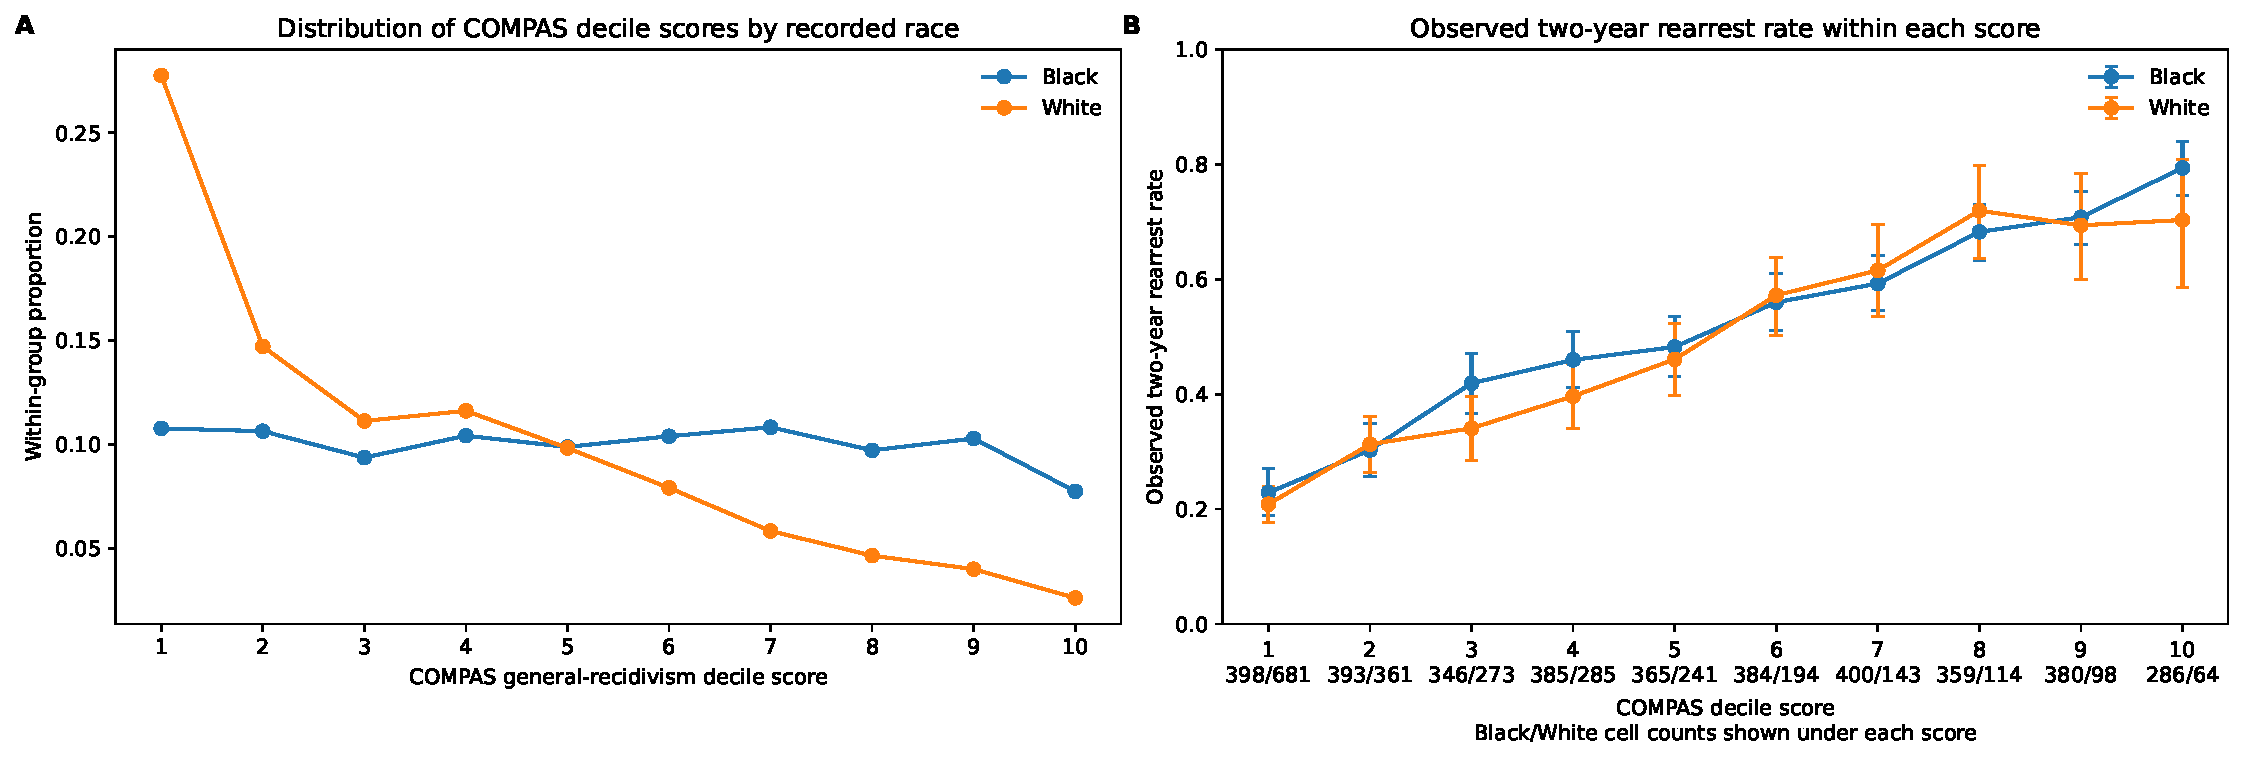
\includegraphics[width=\textwidth]{figure2.pdf}
\caption{Score distributions and observed outcomes. Panel A shows the within-group distribution of general-recidivism decile scores. Panel B shows observed two-year rearrest rates within each score with pointwise 95\% bootstrap intervals; Black/White cell counts are printed below each score. The decile is not treated as a literal probability forecast.}
\label{fig:score-diagnostics}
\end{figure}

\subsection{Moving the threshold changes the allocation of errors}

At the conventional $t=5$ cutoff, the false-positive rate was 44.85\% for Black defendants and 23.45\% for White defendants, a gap of 21.39 percentage points. The false-negative pattern ran in the opposite direction: 27.99\% for Black defendants and 47.72\% for White defendants, a gap of $-19.74$ percentage points. Positive predictive values were much closer, at 62.97\% and 59.13\%, respectively (Table~\ref{tab:threshold-cost-results}; Figure~\ref{fig:t5}).

\begin{figure}[t]
\centering
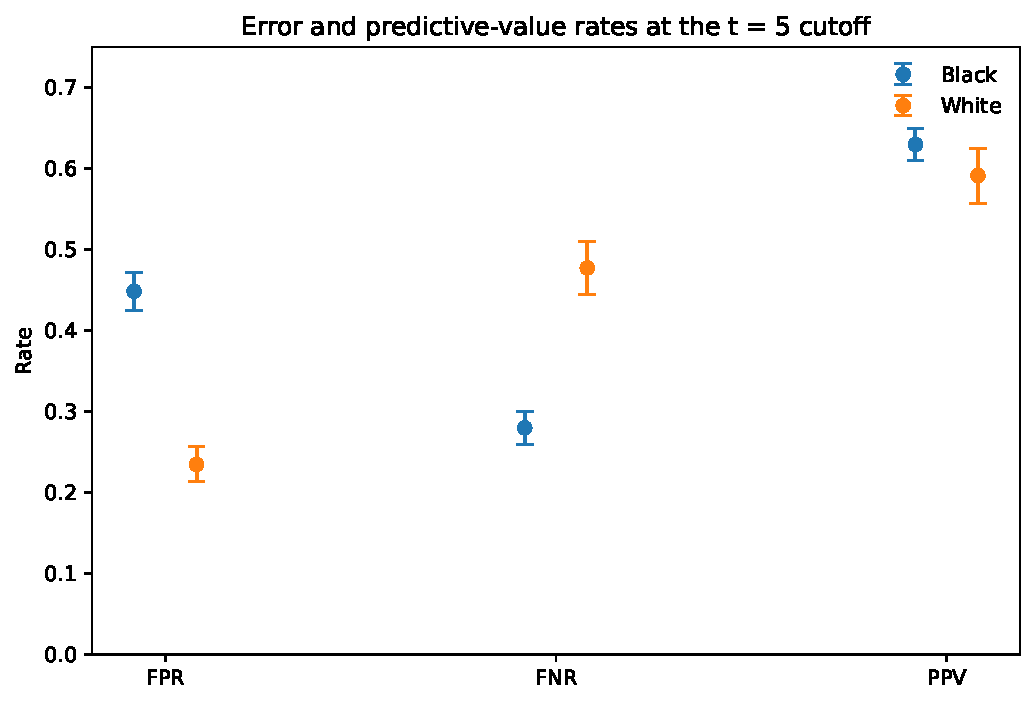
\includegraphics[width=0.72\textwidth]{figure1.pdf}
\caption{Group-specific false-positive rate, false-negative rate, and positive predictive value at the $t=5$ common cutoff. Points are estimates and bars are pointwise 95\% bootstrap intervals.}
\label{fig:t5}
\end{figure}

These differences were not unique to the $t=5$ cutoff. Increasing the common threshold reduced false-positive rates and increased false-negative rates for both groups, while also reducing the share classified as higher risk. The relative allocation of errors, however, changed with the threshold rather than disappearing. At $t=8$, for example, the Black-minus-White FPR gap was still $+10.38$ percentage points, while the FNR gap remained $-18.79$ percentage points. The corresponding PPV gap was only $+1.64$ percentage points (Table~\ref{tab:threshold-cost-results}; Figures~\ref{fig:threshold-consequences}--\ref{fig:gaps}).

\begin{table}[p]
\centering
\caption{Core threshold results and cost-sensitive optimal thresholds}
\label{tab:threshold-cost-results}
\small
\setlength{\tabcolsep}{3pt}
\begin{threeparttable}
\begin{tabular*}{\textwidth}{@{\extracolsep{\fill}}llrrrrr@{}}
\toprule
\multicolumn{7}{l}{\textit{Panel A. Prespecified common cutoffs}} \\
\midrule
Cutoff & Metric & Black (\%) & White (\%) & B$-$W gap (pp) & 95\% bootstrap CI & B/W ratio \\
$t=5$ & FPR & 44.85 & 23.45 & $+21.39$ & [$+18.13$, $+24.55$] & 1.91 \\
& FNR & 27.99 & 47.72 & $-19.74$ & [$-23.50$, $-16.01$] & 0.59 \\
& PPV & 62.97 & 59.13 & $+3.84$ & [$+0.02$, $+7.77$] & -- \\
$t=8$ & FPR & 15.82 & 5.44 & $+10.38$ & [$+8.37$, $+12.48$] & 2.91 \\
& FNR & 61.02 & 79.81 & $-18.79$ & [$-22.16$, $-15.37$] & 0.76 \\
& PPV & 72.29 & 70.65 & $+1.64$ & [$-4.38$, $+7.61$] & -- \\
\midrule
\multicolumn{7}{l}{\textit{Panel B. Focal cost sensitivity}} \\
\midrule
\multicolumn{2}{l}{$\lambda$ (FP:FN)} & Primary $t^*$ & Aggregate loss & Black loss & White loss & Bootstrap share \\
\multicolumn{2}{l}{0.25 (1:3)} & 2 & 0.1275 & 0.1191 & 0.1401 & 99.62\% \\
\multicolumn{2}{l}{0.50 (1:1)} & 6 & 0.1720 & 0.1791 & 0.1612 & 90.92\% \\
\multicolumn{2}{l}{0.75 (3:1)} & 10 & 0.1150 & 0.1252 & 0.0996 & 87.70\% \\
\bottomrule
\end{tabular*}
\begin{tablenotes}[flushleft]
\footnotesize
\item \textit{Note.} A common threshold applies to both groups: higher risk if $S_i\geq t$. The $t=5$ cutoff separates Low from Medium/High; $t=8$ separates Low/Medium from High. Gaps are signed Black-minus-White percentage-point differences; FPR and FNR ratios use the White rate. Intervals are pointwise 95\% percentile intervals from 5,000 race-stratified bootstrap replicates. Primary $t^*$ minimizes $[\lambda FP+(1-\lambda)FN]/N$ in sample C; group losses use each group's own $N$. Bootstrap share is the percentage of replicates whose minimizing set contains the displayed threshold, so shares may sum above 100\% when minimizers tie. The weight $\lambda$ is a sensitivity parameter, not measured social harm.
\end{tablenotes}
\end{threeparttable}
\end{table}

\subsection{Error-rate disparities persist across nondegenerate thresholds}

Across the interior threshold range, the signed FPR gap remained positive and the FNR gap remained negative, indicating that Black defendants experienced higher false-positive rates while White defendants experienced higher false-negative rates under the same common threshold. Pointwise bootstrap intervals for both gaps remained separated from zero across all interior thresholds ($t=2,\ldots,10$) (Figure~\ref{fig:gaps}).

PPV differences were considerably smaller and less stable. Around the central thresholds, the Black-minus-White PPV gap approached zero, and several pointwise bootstrap intervals crossed zero. This combination---similar ranking discrimination and comparatively small predictive-value differences alongside much larger error-rate differences---illustrates why no single performance statistic determines how classification errors are distributed.

\begin{figure}[tbp]
\centering
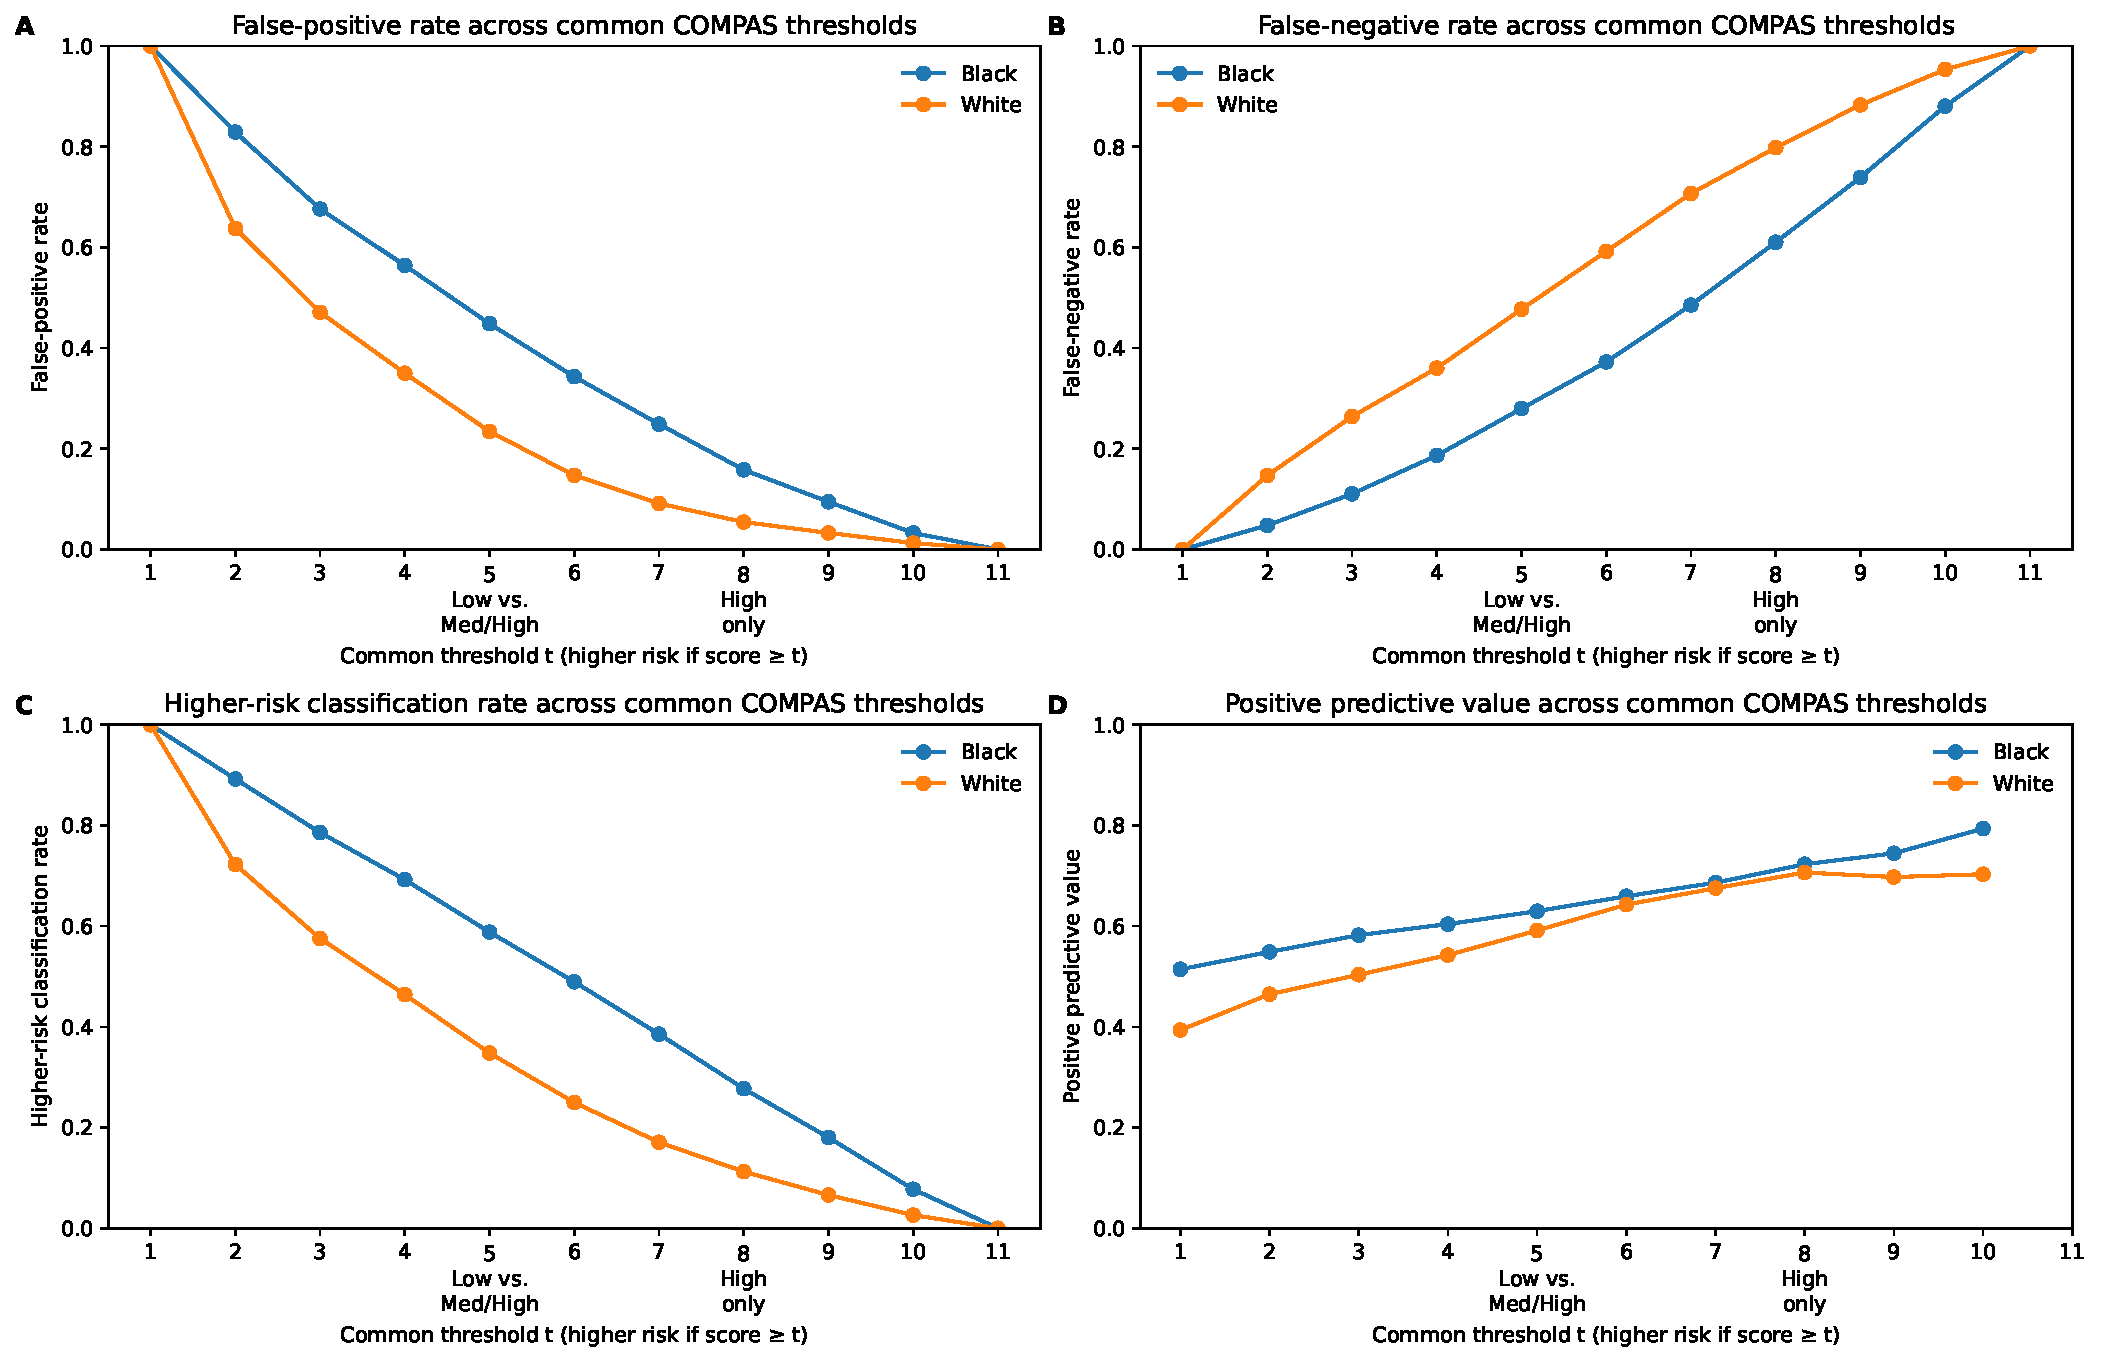
\includegraphics[width=0.97\textwidth]{figure3.pdf}
\caption{Consequences of moving the common threshold. Panels show group-specific FPR, FNR, higher-risk classification rate, and PPV for thresholds $t=1,\ldots,11$. The same threshold is applied to both groups. Endpoints are retained even when PPV or NPV is undefined because no one or everyone is classified higher risk.}
\label{fig:threshold-consequences}
\end{figure}

\begin{figure}[p]
\centering
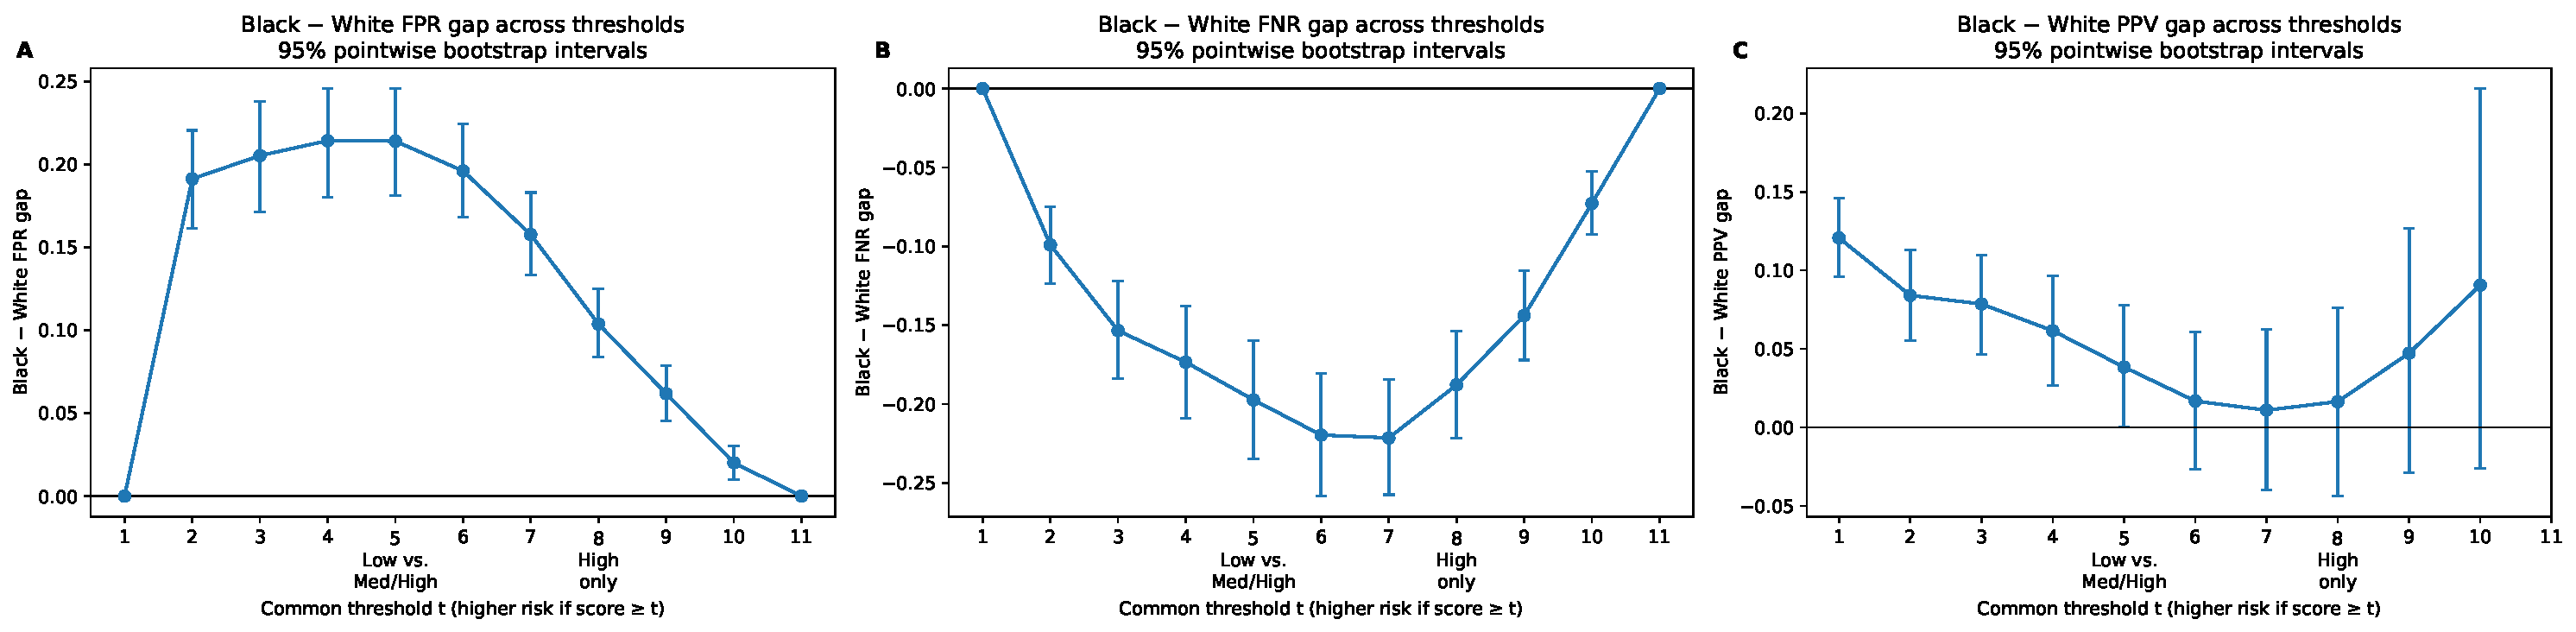
\includegraphics[width=\textwidth]{figure4.pdf}
\caption{Signed Black-minus-White metric gaps across common thresholds. Panels show FPR, FNR, and PPV gaps with pointwise 95\% bootstrap intervals. The horizontal line marks zero. Intervals are descriptive and are not simultaneous or multiple-testing-adjusted.}
\label{fig:gaps}
\end{figure}

\subsection{The loss-minimizing threshold depends strongly on error valuation}

The location of the aggregate loss-minimizing threshold changed sharply with the prespecified error weighting. When false negatives were weighted three times as heavily as false positives ($\lambda=0.25$), the aggregate per-defendant loss was minimized at $t=2$. Under equal weighting ($\lambda=0.50$), the optimum moved to $t=6$. When false positives received three times the weight of false negatives ($\lambda=0.75$), the optimum moved to $t=10$ (Table~\ref{tab:threshold-cost-results}; Figure~\ref{fig:cost}).

The displayed threshold belonged to the complete minimizing set in 99.62\%, 90.92\%, and 87.70\% of defendant-level bootstrap replicates at $\lambda=0.25,0.50,$ and $0.75$, respectively.

As a prespecified population robustness check, the focal aggregate optima were unchanged in sample R ($t^*=2,6,10$ at $\lambda=0.25,0.50,0.75$); the complete sample R and sample C minimizing sets differed at only 5 of 101 grid weights, each by one adjacent threshold.

The prespecified class-conditional loss check produced a different answer at equal weighting. At $\lambda=0.50$, the per-defendant loss selected $t=6$, whereas the class-conditional loss selected $t=5$ (Figure~\ref{fig:supp-loss}). At $\lambda=0.25$ and $0.75$, both specifications selected $t=2$ and $t=10$, respectively.

Aggregate optimality also did not imply equal modeled burden across groups. At the equal-weight optimum ($t=6$), for example, group-specific weighted error loss was 0.1791 for Black defendants and 0.1612 for White defendants. At $\lambda=0.75$ and $t=10$, the corresponding values were 0.1252 and 0.0996. These quantities are sensitivity measures rather than estimates of social harm, but they show that minimizing aggregate loss and evaluating its distribution across groups are distinct questions.

\begin{figure}[p]
\centering
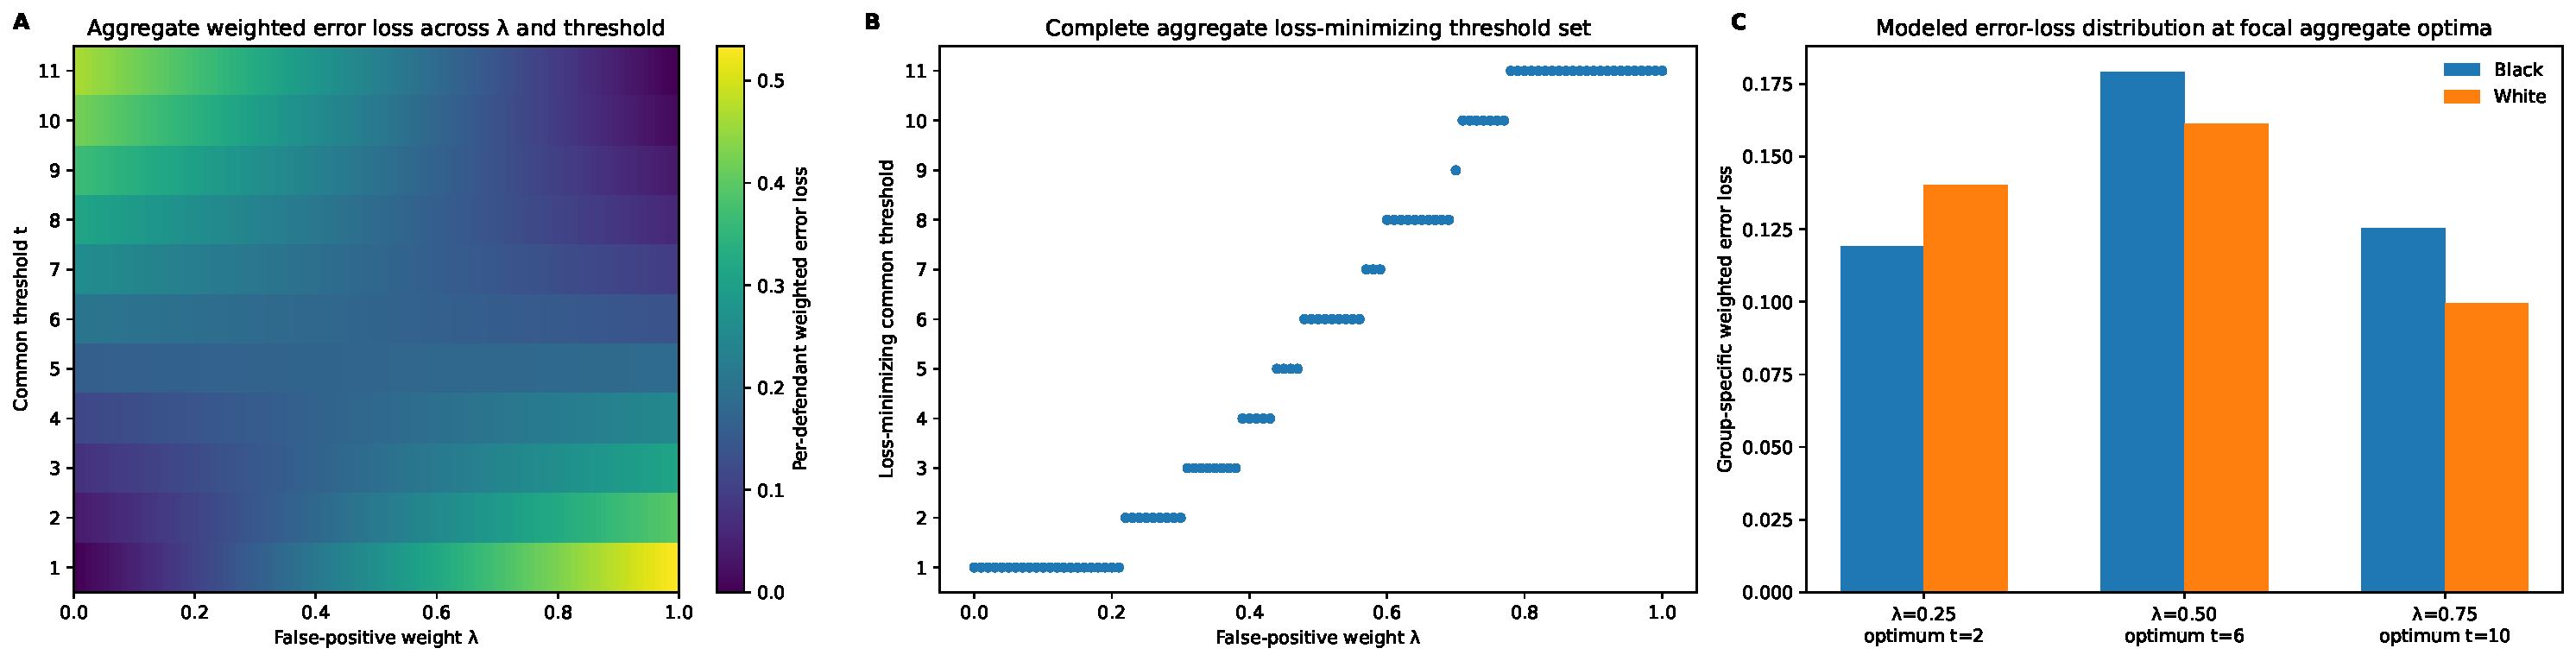
\includegraphics[width=\textwidth]{figure5.pdf}
\caption{Cost sensitivity and conditional optima. Panel A maps per-defendant aggregate weighted error loss over $\lambda$ and the common threshold. Panel B shows the complete minimizing set at every grid weight. Panel C shows group-specific weighted error loss at the focal aggregate optima. The loss is a sensitivity device, not a measure of realized social harm.}
\label{fig:cost}
\end{figure}

\FloatBarrier

\section{Discussion: Institutional Accountability}

The analysis does not reconstruct a historical judicial decision. It does, however, show what a prospective user of a threshold-based rule would have to choose and explain. Table~\ref{tab:accountability-framework} proposes a record for that purpose. Its central object is the decision rule, including its loss definition and permitted consequence, rather than an isolated score-performance statistic.

\subsection{What changes between adjacent thresholds}

Consider the move from $t=5$ to $t=6$ in sample C. All 606 defendants with a score of 5 switch from the analytical higher-risk category to the lower-risk category. Relative to $t=5$, this produces 319 fewer false positives and 287 more false negatives: 32 fewer classification errors in total. At equal error weights, the primary per-defendant loss falls only from 0.1746 to 0.1720. The Black-minus-White FPR gap narrows from 21.39 to 19.60 percentage points, while the FNR gap widens in magnitude from 19.74 to 21.97 percentage points (Figures~\ref{fig:threshold-consequences}--\ref{fig:gaps}). The changes are descriptive consequences of two specified rules applied to the historical data; they are not observed changes in detention, sentencing, or any other legal outcome.

The comparison makes the decision problem less abstract. A small improvement in an aggregate objective accompanies a change in which errors occur and how their rates differ across groups. For illustration, if a jurisdiction proposed to use a higher-risk classification only to trigger additional review, moving from $t=5$ to $t=6$ would avoid that trigger for 319 people not observed to be rearrested and also for 287 people later observed to be rearrested. The institution would need to explain what the review actually does before treating either change as beneficial or harmful. This is a hypothetical use of the classification, not a claim about Broward County practice.

\subsection{The objective also requires a choice}

The class-conditional check identifies a choice within the word ``equal.'' At $\lambda=.50$, the primary objective counts errors over all defendants and selects $t=6$; the alternative normalizes separately by the observed non-rearrested and rearrested pools and selects $t=5$ (Figure~\ref{fig:supp-loss}). Both are transparent calculations, but they answer different questions. A claim that a threshold is ``optimal'' should therefore name the population, outcome, loss normalization, and weights before presenting the selected cutoff.

The unequal group-specific losses at the focal aggregate optima add a separate distributive question. For example, at $\lambda=.50$ and $t=6$, modeled weighted error loss is 0.1791 for Black defendants and 0.1612 for White defendants (Table~\ref{tab:threshold-cost-results}). These figures are not measures of realized social harm. They show why choosing an aggregate objective does not end an assessment of how its errors are distributed.

\subsection{A record for institutional review}

Table~\ref{tab:accountability-framework} organizes a proposed record around four linked tasks. The institution first identifies who authorized a particular rule and what consequence the classification may influence. It then places the adjacent-threshold comparison and the alternative equal-weight optima beside that rule, so the reasons for the selected objective can be assessed against visible alternatives. Recording those choices matters only if an affected person can also identify the rule applied in an individual case, challenge erroneous inputs or applicability, and obtain a reasoned review with a remedy. These are proposed accountability conditions, not findings about historical COMPAS deployment or a complete statement of legal requirements.

\begin{table}[t]
\centering
\caption{Operational accountability framework for threshold-based algorithmic decisions}
\label{tab:accountability-framework}
\small
\setlength{\tabcolsep}{4pt}
\renewcommand{\arraystretch}{1.16}
\begin{threeparttable}
\begin{tabular}{@{}>{\raggedright\arraybackslash}p{0.18\textwidth}>{\raggedright\arraybackslash}p{0.40\textwidth}>{\raggedright\arraybackslash}p{0.36\textwidth}@{}}
\toprule
Module & Proposed record or disclosure & What this analysis illustrates \\
\midrule
\textbf{Decision specification} & Name authority, outcome/horizon, population, score/version, threshold, and permitted consequence & Moving from $t=5$ to $t=6$ reclassifies all 606 score-5 defendants \\
\addlinespace
\textbf{Error accounting} & Publish counts, denominators, subgroup rates, gaps, uncertainty, and threshold sensitivity & The move yields 319 fewer FP and 287 more FN; the FPR gap narrows while the FNR gap widens \\
\addlinespace
\textbf{Institutional justification} & Record the loss definition, error weights, alternatives, reasons, and revision triggers & At $\lambda=.50$, per-defendant loss selects $t=6$; class-conditional loss selects $t=5$ \\
\addlinespace
\textbf{Individual contestability} & Enable challenge to inputs, applicability, score/version/threshold, consequence, and reasons & Aggregate results cannot establish the effect of a classification in an individual case \\
\bottomrule
\end{tabular}
\end{threeparttable}
\end{table}

\FloatBarrier

\section{Limitations}

First, the outcome is observed two-year rearrest, not true offending or a complete measure of recidivism. Rearrest is shaped by policing intensity, surveillance, reporting, charging, and record-linkage processes, so the label may reflect institutional practices as well as underlying conduct. ProPublica's audit also estimated a 3.75\% record-matching error rate, with an interval of approximately $\pm1.8$ percentage points \citep{larson2016}. The reported metrics therefore describe the score's relationship to the observed rearrest label, not its accuracy against an unobserved ground truth of offending.

Second, the data are historical and local. They concern defendants in Broward County, Florida, scored principally in 2013--2014, and cannot establish current performance in Broward County, performance in other jurisdictions, or the behavior of other risk instruments. The public data contain recorded scores and outcomes but not the complete proprietary COMPAS formula, training data, or institutional implementation rules. This study evaluates the available historical outputs; it is not an audit of the current COMPAS system or of contemporary deployment practice.

Third, the source categories \texttt{African-American} and \texttt{Caucasian}, displayed here as Black and White, are recorded administrative labels rather than self-identified racial identities. The primary comparison omits inferential analysis for smaller recorded groups and does not address intersectional patterns. Moreover, the reported gaps are descriptive associations among recorded race, scores, and observed outcomes. They do not identify a causal effect of race or isolate the mechanisms that produced the differences.

Fourth, the threshold sweep is an analytical sensitivity exercise rather than a reconstruction of historical deployment. Applying common thresholds $t=1,\ldots,11$ shows how classification consequences would change under alternative rules; it does not claim that Broward County judges or agencies actually used each threshold, used the score as a binding binary classifier, or attached a particular consequence to every higher-risk classification. Because COMPAS scores are discrete, only a finite set of common thresholds is available, and neighboring values of $\lambda$ may therefore yield the same minimizing threshold set. The results characterize the implications of specified rules, not the decisions of particular officials.

Fifth, $\lambda$ is a prespecified sensitivity parameter, not a measured social-welfare weight. The movement of the aggregate optimum from $t=2$ to $t=6$ to $t=10$ demonstrates dependence on the stated objective, but it does not show that any $\lambda$ is legally, morally, or institutionally appropriate. The loss function does not monetize individual harm, and group-specific weighted error loss is not realized social harm. More generally, neither an aggregate optimum nor any single performance metric settles institutional legitimacy.

Finally, the 5,000-replicate race-stratified defendant-level bootstrap captures sampling variation conditional on the observed dataset, prespecified analysis, and specified resampling scheme. It does not incorporate systematic label bias, record-linkage error, model drift, policy change, uncertainty about institutional use, or external-validity uncertainty. The reported metric-gap intervals are pointwise rather than simultaneous, and optimal-threshold membership frequencies measure stability under this resampling scheme rather than total uncertainty about the decision rule.

\section{Conclusion}

In these historical COMPAS data, similar Black and White ranking discrimination coexists with substantial, oppositely signed classification-error gaps. The adjacent $t=5$ and $t=6$ rules expose a concrete exchange: 319 fewer false positives for 287 more false negatives in the comparison sample, with a small improvement in equal-weight per-defendant loss. At the same numerical weight, a class-conditional objective selects $t=5$ instead of $t=6$. Thus, even the definition of an ``equal-weight optimum'' depends on how errors are counted.

The study cannot identify an appropriate legal consequence, a morally correct error weight, or the threshold used in historical judicial practice. It can identify what a prospective institutional decision would need to make explicit: the population and outcome, the threshold, the loss definition and weights, the distribution of errors, the permitted use of the classification, and a route to review and remedy. The proposed accountability record makes those choices open to justification rather than attributing them to the score itself.

\section*{Declaration of Generative AI Use}

Generative AI tools were used for grammar and language editing, structural feedback, revision of selected passages, and assistance with literature searches.

\bibliographystyle{plainnat}
\bibliography{references}

\clearpage
\appendix
\section{Supplemental robustness figures}

\begin{figure}[H]
\centering
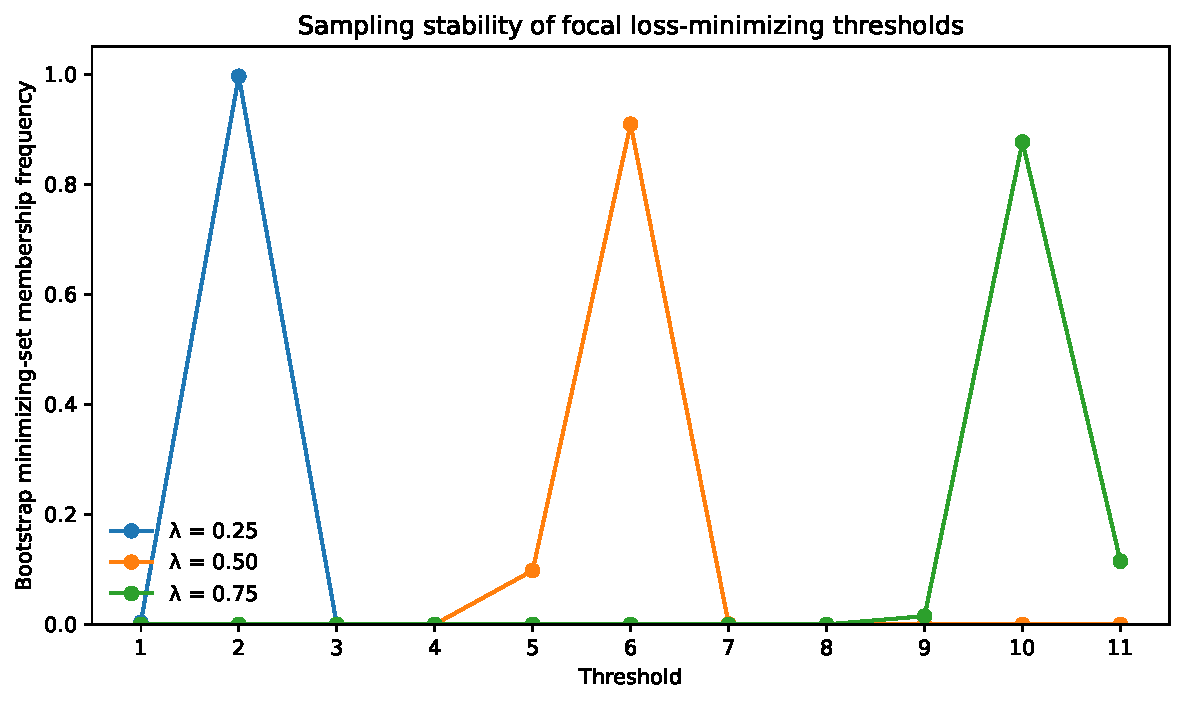
\includegraphics[width=0.82\textwidth]{supplement_bootstrap_optimal_membership.pdf}
\caption{Bootstrap minimizing-set membership frequencies at the three focal error weights. A replicate may have tied minimizers, so threshold membership frequencies at a given weight need not sum to 100\%.}
\label{fig:supp-bootstrap}
\end{figure}

\begin{figure}[H]
\centering
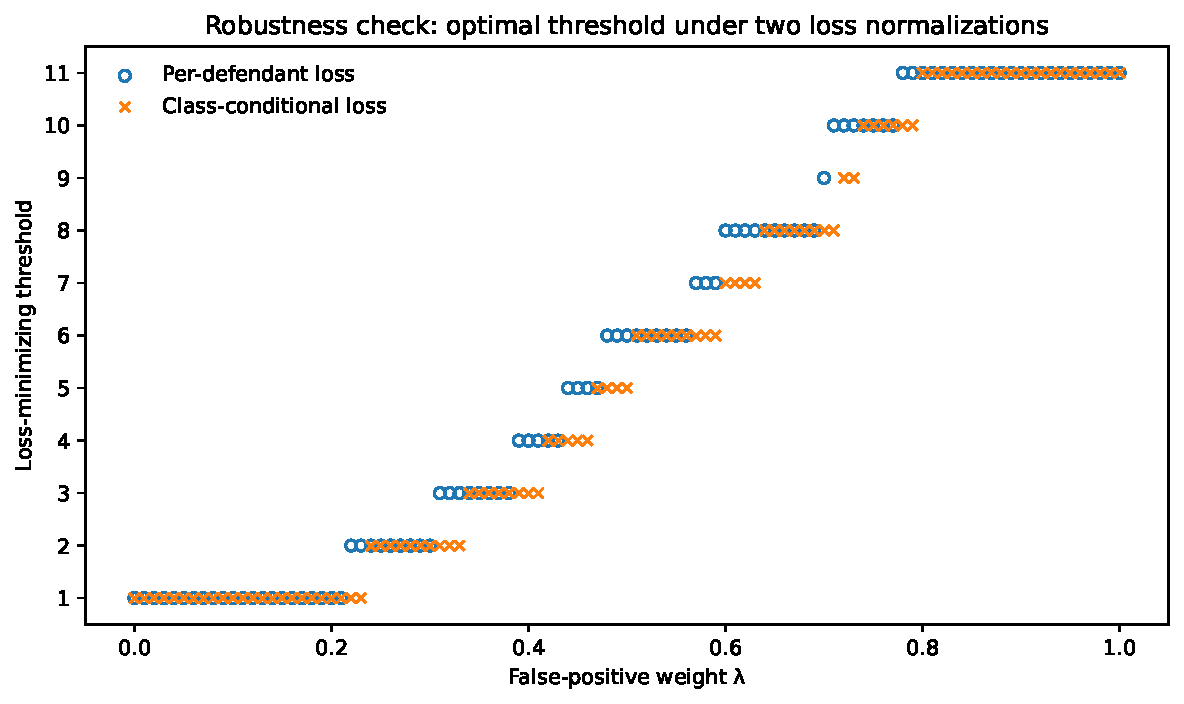
\includegraphics[width=0.82\textwidth]{supplement_robustness_optimal_thresholds.pdf}
\caption{Complete loss-minimizing threshold sets under the per-defendant primary loss and the class-conditional robustness loss across the full $\lambda$ grid. Hollow and crossed markers preserve coincident minimizers.}
\label{fig:supp-loss}
\end{figure}

\end{document}
